\documentclass[aps,prb,showpacs,amsmath,twocolumn,amssymb,superscriptaddress]{revtex4-2}
%\documentclass[aps,prb,showpacs,twocolumn,amsmath,amssymb,superscriptaddress]{revtex4-2}
%\bibliographystyle{apsrev4-2}

\usepackage{tabularx}
\usepackage{bm}
%\usepackage[demo]{graphicx}
\usepackage{graphicx}
\usepackage{tikz}
%\usepackage{setspace}
%\setstretch{3}

\usepackage{hyperref}
\hypersetup{colorlinks=true,urlcolor= blue,citecolor=blue,linkcolor= blue,bookmarks=true,bookmarksopen=false}

\usepackage{color}

\usepackage{amsmath,mathtools}
\usepackage{multirow}
\usepackage{dcolumn}
\usepackage{amssymb,amscd,xypic,bm,wasysym}
\usepackage{float}
\usepackage{cleveref}
\usepackage[caption=false,position=top,captionskip=0pt,farskip=0pt]{subfig}
\captionsetup[subfigure]{justification=raggedright,singlelinecheck=false}

\newcommand{\Red}[1]{\textcolor{red}{#1}}
\newcommand{\Blue}[1]{\textcolor{blue}{#1}}
%\newcommand{\vb}[1]{\boldsymbol{#1}}
\usepackage{soul}

% reset vec and hat style to a bold type
\let\oldhat\hat
\renewcommand{\hat}[1]{\oldhat{\mathbf{#1}}}
\renewcommand{\vec}[1]{\mathbf{#1}}
% stretches the vertical spacing of arrays/matrices
\renewcommand{\arraystretch}{1.5}
\setlength{\jot}{10pt}

\newcommand{\ham}{\mathcal{H}}
\newcommand{\cc}{c^{\dagger}}
\newcommand{\de}{\Delta}

\begin{document}

\title{Superconducting triangular islands as a platform for manipulating Majorana zero modes}

\author{Aidan Winblad}
\affiliation{Department of Physics, Colorado State University, Fort Collins, CO 80523, USA}

\author{Hua Chen}
\affiliation{Department of Physics, Colorado State University, Fort Collins, CO 80523, USA}
\affiliation{School of Advanced Materials Discovery, Colorado State University, Fort Collins, CO 80523, USA}

\begin{abstract}
Current proposals on topological quantum computation (TQC) based on Majorana zero modes (MZM) have mostly been focused on coupled-wire architecture which can be challenging to implement experimentally. To explore alternative building blocks of TQC, in this work we study the possibility of obtaining robust MZM at the corners of triangular superconducting islands, which often appear spontaneously in epitaxial growth. We first show that a minimal three-site triangle model of spinless $p$-wave superconductor allows MZM to appear at different pairs of vertices controlled by a staggered vector potential, which may be realized using coupled quantum dots and can be extended to larger triangular networks. For systems with less fine-tuned parameters, we suggest an alternative structure of a ``hollow" triangle subject to inhomogeneous supercurrents, in which MZM generally appear when two of the edges are in a different topological phase from the third. We also discuss the robustness of MZM in various possible experimental realizations of the triangular islands.
\end{abstract}


\maketitle


\section{Introduction}
For more than twenty years, Majorana zero modes (MZM) in condensed matter systems have been highly sought after due to their potential for serving as building blocks of topological quantum computation, thanks to their topological robustness against decoherence and non-Abelian exchange statistics \cite{ivanovNonAbelianStatisticsHalfQuantum2001, kitaevFaulttolerantQuantumComputation2003, nayakNonAbelianAnyonsTopological2008, aliceaNonAbelianStatisticsTopological2011, aasenMilestonesMajoranaBasedQuantum2016}. Theoretically, MZM were originally proposed to be found in half-quantum vortices of two-dimensional (2D) topological \textit{p}-wave superconductors and at the ends of 1D spinless \textit{p}-wave superconductors \cite{readPairedStatesFermions2000, kitaevUnpairedMajoranaFermions2001}.
Whether a pristine \textit{p}-wave superconductor {\bf [REF]} has been found is still under debate. However, innovative heterostructures proximate to ordinary $s$-wave superconductors have been proposed to behave as effective topological superconductors in both 1D and 2D. These, for example, \Red{semiconductor nanowires subject to magnetic fields}\cite{mourikSignaturesMajoranaFermions2012, rokhinsonFractionalJosephsonEffect2012, dengAnomalousZeroBiasConductance2012}, ferromagnetic atomic spin chains \cite{choyMajoranaFermionsEmerging2011, brauneckerInterplayClassicalMagnetic2013, klinovajaTopologicalSuperconductivityMajorana2013,nadj-pergeObservationMajoranaFermions2014,schneiderPrecursorsMajoranaModes2022}, 3D topological insulators \cite{fuSuperconductingProximityEffect2008, hosurMajoranaModesEnds2011, potterEngineeringMathitipSuperconductor2011, veldhorstMagnetotransportInducedSuperconductivity2013}, quantum anomalous Hall insulators \cite{chenQuasionedimensionalQuantumAnomalous2018, zengQuantumAnomalousHall2018, xieCreatingLocalizedMajorana2021}, 2D Rashba electron gas with a perpendicular Zeeman field \cite{oregHelicalLiquidsMajorana2010, sauGenericNewPlatform2010, lutchynSearchMajoranaFermions2011, potterTopologicalSuperconductivityMajorana2012, nadj-pergeProposalRealizingMajorana2013}, \Red{metallic ferromagnets}, and \Red{planar Josephson junctions} \cite{black-schafferMajoranaFermionsSpinorbitcoupled2011, pientkaSignaturesTopologicalPhase2013, hellTwoDimensionalPlatformNetworks2017, scharfTuningTopologicalSuperconductivity2019}, etc. It has been a challenging task to decisively confirm the existence of MZM in the various experimental systems due to other competing mechanisms that can potentially result in similar features as MZM do in different probes \cite{xuExperimentalDetectionMajorana2015, albrechtExponentialProtectionZero2016, sunMajoranaZeroMode2016, wangEvidenceMajoranaBound2018, jackObservationMajoranaZero2019, fornieriEvidenceTopologicalSuperconductivity2019, renTopologicalSuperconductivityPhasecontrolled2019, mannaSignaturePairMajorana2020}. Other proposals for constructing Kitaev chains through a bottom-up approach, based on, e.g. \Red{magnetic tunnel junctions proximate to spin-orbit-coupled superconductors}, and \Red{quantum dots coupled through superconducting links} are therefore promising. In particular, the recent experiment of a designer minimal Kitaev chain based on two quantum dots coupled through tunable crossed Andreev reflections (CAR) offers a compelling route towards MZM platforms based on exactly solvable building blocks.
%A new potential measurement may soon help confirm the identity of MZMs using a quantum dot and  \cite{fengProbingRobustMajorana2022}.

In parallel with the above efforts of realizing MZM in different materials systems, scalable architectures for quantum logic circuits based on MZM have also been intensely studied over the past decades. A major proposal among these studies is to build networks of T-junctions, which are minimal units for swapping a pair of MZM hosted at different ends of a junction, that allow braiding-based TQC \cite{karzigScalableDesignsQuasiparticlepoisoningprotected2017}. Alternatively, networks based on coupled wires forming the so-called tetrons and hexons, aiming at measurement-based logic gate operations, have also been extensively investigated. To counter the technical challenge of engineering networks with physical wires or atomic chains, various ideas based on effective Kitaev chains, such as quasi-1D systems in thin films \cite{potterMultichannelGeneralizationKitaev2010}, cross Josephson junctions \cite{zhouPhaseControlMajorana2020}, scissor cuts on a QAHI \cite{xieCreatingLocalizedMajorana2021}, and rings of magnetic atoms {\bf [REF]}, etc. have been proposed. However, due to the same difficulty of obtaining or identifying genuine MZM in quasi-1D systems mentioned above, it remains unclear how practical these strategies are in the near term.

\Red{Higher-order topological superconductors and corner MZM}

In this work, we propose an alternative structural unit for manipulating MZM, triangular superconducting islands, motivated by the above challenges associated with wire geometries and by the fact that triangular islands routinely appear spontaneously in epitaxial growth \cite{pietzschSpinResolvedElectronicStructure2006} on close-packed atomic surfaces. We first show that a minimal ``Kitaev triangle'' consisting of three sites hosts MZM at different pairs of vertices controlled by Peierls phases on the three edges, which can be readily realized using quantum dots. To generalize the minimal model to other means of engineering topologically equivalent triangles, we study the topological phase transitions of quasi-1D ribbons driven by Peierls phases, which can be created by magnetic fields or supercurrents \cite{romitoManipulatingMajoranaFermions2012, takasanSupercurrentinducedTopologicalPhase2022}, and use the resulting phase diagram as a guide to construct finite-size triangles with a hollow interior that host MZM. In the end we discuss possible experimental systems that can realize our proposals and scaled-up networks of triangles for implementing MZM-based logic gate operations. 

\section{A minimal Kitaev triangle model}

In this section we present an exactly solvable minimal model (\Red{not analytically solvable though--perhaps solvable with the help of symmetry}) with three sites forming a ``Kitaev triangle" that can host MZM at different pairs of vertices controlled by Peierls phases on the triangle edges. The Bogoliubov-de Gennes (BdG) Hamiltonian includes complex hopping and $p$-wave pairing between three spinless fermions forming an equilateral triangle ({\bf Fig. XXX--Add a schematic figure}):
\begin{equation}
  \ham = \sum_{\langle j l \rangle} (-te^{i\phi_{jl}}\cc_{j} c_l + \de e^{i\theta_{jl}} c_{j} c_l + {\rm h.c.}) - \sum_{j} \mu \cc_j c_j,
\end{equation}
where $t$ is the hopping amplitude, $\de$ is the amplitude of the (2D) $p$-wave pairing, $\mu$ is the chemical potential, $\theta_{jl}$ is the polar angle of $\mathbf r_{jl} = \mathbf r_l - \mathbf r_j$ (the $x$ axis is chosen to be along $\mathbf r_{12}$), consistent with $\{c^\dag_l, c^\dag_j\} = 0$. $\phi_{jl}$ is the Peierls phase due to a bond-dependent vector potential $\mathbf A$ to be specified below: 
\begin{eqnarray}
\phi_{jl} = \dfrac{e}{\hbar} \int_{\mathbf r_j}^{\mathbf r_{l}} \vec{A} \cdot d\vec{l} = -\phi_{lj}
\end{eqnarray}
where $e>0$ is the absolute value of the electron change. {\bf I changed the order of labeling $j,l$ etc. above. I understand that it may be more natural to think of $c_j^\dag c_l$ as hopping from $l$ to $j$, but people are more used to write the labels from left to right. For the pairing term this is consistent with \cite{kitaevUnpairedMajoranaFermions2001}.} To get the conditions for having MZM in this model we rewrite $\mathcal{H}$ in the Majorana fermion basis $a_{j} = c_j + c^\dag_j$, $b_j = \frac{1}{i}(c_j - c^\dag_j)$ \cite{supp}:
\begin{align}\label{eq:H3M}
    \ham =  -\dfrac{i}{2} \sum_{\langle j l \rangle} \Big[&\left(t\sin\phi_{jl}-\de\sin\theta_{jl}\right) a_j a_l \\\nonumber
  +&\left(t\sin\phi_{jl}+\de\sin\theta_{jl}\right) b_j b_l  \\\nonumber
  +&\left(t\cos\phi_{jl} - \de\cos\theta_{jl}\right) a_j b_l  \\\nonumber
  -&\left(t\cos\phi_{jl}+\de\cos\theta_{jl}\right) b_j a_l\Big]  -\dfrac{i\mu}{2} \sum_j  a_j b_j
\end{align}
For concreteness we consider the Kitaev limit $t=\de$, $\mu=0$, and choose $\phi_{12} = 0$ so that sites 1 and 2 alone form a minimal Kitaev chain with $\mathcal{H}_{12} = itb_1a_2$ and hosting MZM $a_1$ and $b_2$. In order for the MZM to persist in the presence of site 3, one can choose $\phi_{23}$ and $\phi_{31}$ so that all terms involve these Majorana operators cancel out. For example, consider the $2-3$ bond, for which $\theta_{23} = 2\pi/3$, we require
\begin{align}
  \left(\sin\phi_{23} + \sin\frac{2\pi}{3}\right) b_2 b_3 =\left(\cos\phi_{23} + \cos\frac{2\pi}{3}\right)b_2 a_3 = 0
\end{align}
which means $\phi_{23} = -\pi/3$. Similarly one can find $\phi_{31} =-\phi_{13} = -\pi/3$. The three Peierls phases can be realized by the following staggered vector potential
\begin{equation}
  \vec{A} =\left[1-2\Theta(x)\right]\frac{2 \pi}{3\sqrt{3}a} \hat{y} 
\end{equation}
where $\Theta(x)$ is the Heavisde step function. In fact, using a uniform $\vec{A} =\frac{2 \pi}{3\sqrt{3}a} \hat{y}$, which corresponds to $\phi_{23} = -\pi/3 = -\phi_{31}$ also works, since the existence of $a_1$ is unaffected by $\phi_{23}$. However, in this case the counterpart of $b_2$ is not localized on a single site. For the same reason, the above condition for MZM localized at triangle corners can be generalized to Kitaev chains forming a triangular loop, as well as to finite-size triangles of 2D spinless $p$-wave superconductors in the Kitaev limit, as the existence of $a_1$ and $b_2$ are only dictated by the vector potential near the corresponding corners. It should be noted that in the latter case, 1D Majorana edge states will arise when the triangle becomes larger, and effectively diminishes the gap that protects the corner MZM {\bf Add a figure showing a larger triangle in \cite{supp}}. On the other hand, for the longer Kitaev chain, due to the potential practical difficulty of controlling further-neighbor hopping and pairing amplitudes, it is better to resort to the approach of controlling the individual topological phases of the three edges which will be detailed in the next section. 

We next show that the minimal Kitaev triangle suffices to demonstrate braiding of MZM. To this end we consider a closed parameter path linearly interpolating between the following sets of values of $\phi_{jl}$:
\begin{eqnarray}
    (\phi_{12},\phi_{23},\phi_{31}) &=& \left(0,-\frac{\pi}{3},-\frac{\pi}{3}\right ) \equiv \bm \phi_1 \\\nonumber
    &\rightarrow& \left(-\frac{\pi}{3},-\frac{\pi}{3},0 \right) \equiv \bm \phi_2 \\\nonumber
    &\rightarrow& \left(-\frac{\pi}{3},0,-\frac{\pi}{3} \right) \equiv \bm \phi_3 \\\nonumber
    &\rightarrow& \bm \phi_1
\end{eqnarray}
It is straightforward to show that at $\bm \phi_{2}$ and $\bm \phi_3$ there are MZM located at sites $3,1$ and $2,3$, respectively. Therefore the two original MZM at sites $1,2$ should switch their positions at the end of the adiabatic evolution. 

\begin{figure}[ht]
	\centering
	\subfloat[]{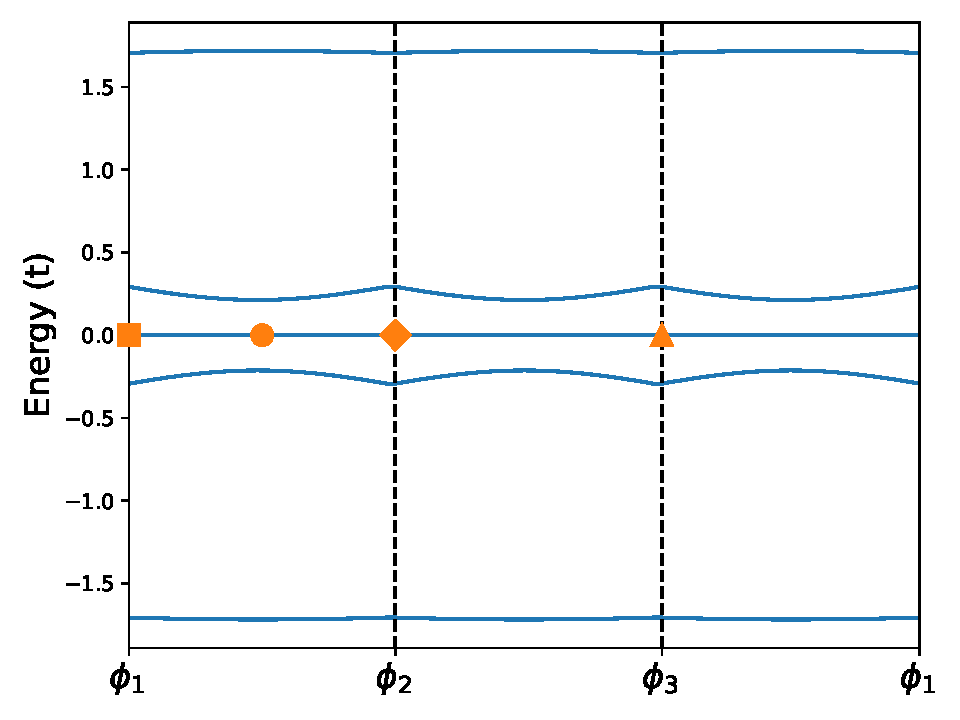
\includegraphics[width=2.1 in]{3eigval.png}}\\
	\subfloat[]{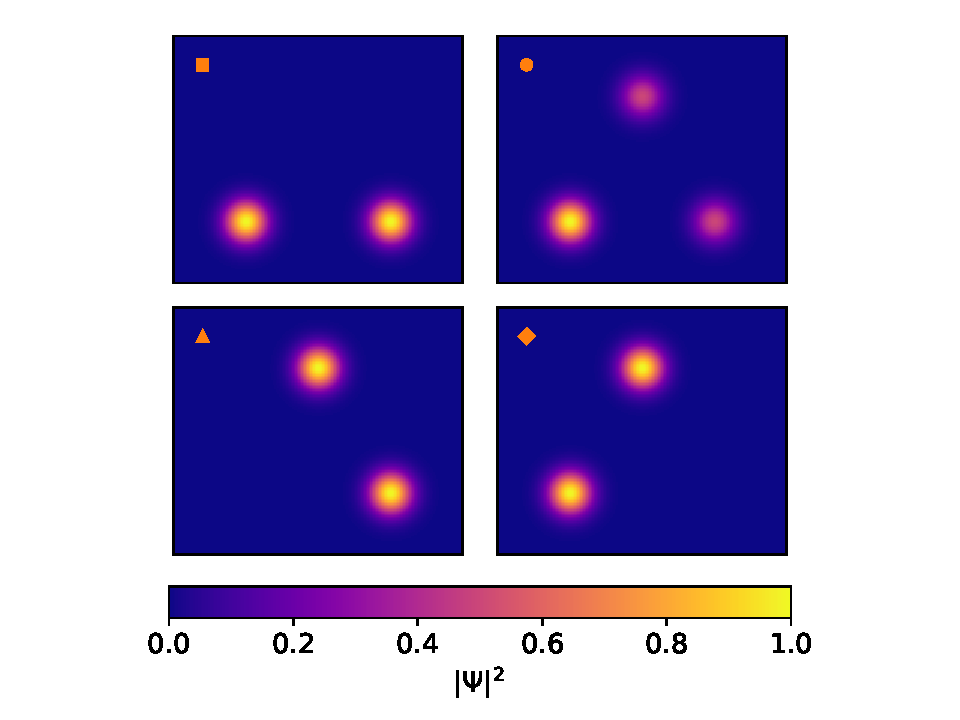
\includegraphics[width=2.8 in]{3eigvec.png}}
	\caption{(a) Evolution of the eigenvalues of the 3-site Kitaev triangle along the closed parameter path for $\phi$ on the three edges. (b) MZM wavefunctions at different points of the parameter path.} 
	\label{fig:3eig}
\end{figure}

\Red{Indeed, Fig.~\ref{fig:3eig} shows that the MZM stays at zero energy throughout the parameter path that interchanges their positions. To show that such an operation indeed realizes braiding, we explicitly calculate the many-body Berry phase of the evolution \cite{aliceaNonAbelianStatisticsTopological2011,Li_2016}.}


In comparison to the minimum T-junction model with four sites \cite{aliceaNonAbelianStatisticsTopological2011}, our Kitaev triangle model only requires three sites to achieve braiding between two MZM, and is potentially also easier to engineer experimentally. In the next section we will show that a more mesoscopic hollow-triangle structure can achieve qualitatively the same result and may be preferred in other materials platforms.

\section{Topological phase diagram of a finite width ribbon}

Kitaev had noted one could still get a topological phase for $-2t<\mu<2t$ and MZMs hosting at the interface of differing topologies \cite{kitaevUnpairedMajoranaFermions2001}.
We would also like to find a range of chemical potentials and vector potential strengths that result in a topologically nontrivial phase.
As a last note, any odd-function vector potential field can achieve exact MZMs on the bottom two vertices of a triangular island.
We only consider constant vector potentials in the next section to allow for a fourier transform of the ribbons main axis.


MZMs can be hosted at the end points of a chain with finite width as with a Josephson-junction or other thin films, provided the width is much smaller than the Majorana fermion decay length \cite{black-schafferMajoranaFermionsSpinorbitcoupled2011, pientkaSignaturesTopologicalPhase2013, hellTwoDimensionalPlatformNetworks2017, scharfTuningTopologicalSuperconductivity2019, potterMultichannelGeneralizationKitaev2010}.
Expanding on these ideas we would like to induce a topological phase transition for an infinite triangular lattice ribbon.
This will help create an argument using bulk-edge correspondence to inform how MZMs will host at the interfaces of triangular island edges, i.e. their corners.

Starting from Eq. \ref{eq: Peierls Hamiltonian} and since we are interested how a finite width ribbon along the $x$-axis behaves in a constant vector field we will fourier transform along the $x$-axis only.
Pick the following transform to be
\begin{equation}
  \cc_{m,n} = \dfrac{1}{\sqrt{N}} \sum_{k} \cc_{k,n} e^{i \vec{k}\cdot\vec{r}_m}
\end{equation}
where $\vec{k}=k\hat{x}$ and $\vec{r}_m = ma\hat{x}$, and for convenience $a$ will be treated as a natural number.
This leads to the following block Hamiltonian
\begin{equation}
  \ham(k) = \dfrac{1}{2} \sum_k \Psi_k^\dagger \left(
    \begin{matrix}
      \epsilon(k) & \delta(k) \\
      \delta^\dagger(k) & -\epsilon(-k)
    \end{matrix} \right)
    \Psi_k.
\end{equation}
The $\epsilon(k)$ block is a tridiagonal with $\epsilon_0(k) = -2t\cos(k+\phi_1) - \mu$ along the diagonal, the upper diagonal is  $\epsilon_1(k) = -t(e^{-i\phi_2}+e^{i(k-\phi_3)})$, and $\epsilon_1^*(k)$ along the lower diagonal.
The $\delta(k)$ block is a tridiagonal with $\delta_0(k) = 2i\de \sin k $ along the diagonal, the upper diagonal is  $\delta_1(k) = -\de (e^{i\theta_2}+e^{i(k+\theta_3)})$, and $-\delta_1(-k)$ along the lower diagonal.
The size of each block is the number of rows along the $y$-axis in a ribbon.

To calculate the Majorana number (\mathcal{M}) the Hamiltonian needs to be in skew-symmetric form.
One such way is to write it in the Majorana fermion basis, the transformation matrix is of the form
\begin{equation}
  u = \dfrac{1}{\sqrt{2}} \left(
  \begin{matrix}
    1 & 1 \\
    -i & i
  \end{matrix} \right)
\end{equation}

To account for the finite number of rows in a ribbon include a tensor product with an identity matrix of the same size, $U = u \otimes I_n$.
We arrive at the skew-symmetric matrix with the following equation
\begin{equation}
  A_{ch} = -i U \ham_{ch} U^{\dagger}.
\end{equation}
The $\mathcal{M}$ of a 1D chain is defined as
\begin{equation}
  \mathcal{M} = \text{sgn}[\text{Pf}(A_{ch})],
\end{equation}
where $\text{Pf}$ stands for the Pfaffian of a skew-symmetric matrix \cite{kitaevUnpairedMajoranaFermions2001}.
We make the claim this satisfies a finite width ribbon as well.
When $\mathcal{M} = -1$, the ribbon is in a nontrivial topology and expect MZMs at its edges.
Sweeping through a range of $A$ for the vector potential we expect to see a gap closing, $\mathcal{M} = 1$, and the system take on a trivial topology, no Majorana zero modes would exist on the edge of a finite ribbon.

To illustrate the importance of bulk-edge correspondence in forming Majorana fermions we will now look at the edges of a hollow triangular island.
We show the top edges can be in a trivial phase while the bottom remains in a nontrivial phase.
In previous papers a constant vector potential was used along the chain's axis \cite{romitoManipulatingMajoranaFermions2012, takasanSupercurrentinducedTopologicalPhase2022}.
We instead use a constant vector potential step function from the previous section centered on a chain with two 60 degree bends, equating it to a equilateral triangle.
Taking a hollow triangular island centered about the y-axis with the following vector potential
\begin{equation}
  \vec{A} = \begin{cases}
            A \hat{y} \quad &x > 0 \\
            -A \hat{y} \quad &x < 0 \\
            \end{cases}
\end{equation}
we examine each edge individually.
When calculating \mathcal{M} the vector potential has symmetry about the ribbon's axis, i.e. $\vec{A}$ pointing in the positive or negative y-axis yields the same result.
Looking at Fig. \ref{fig: triangular-island-vector-potential-divided} we determine each edge's vector potential with respect to its main axis.

\begin{figure}[]
  \begin{tikzpicture}
    \node[inner sep=0pt] (figure) at (0,0){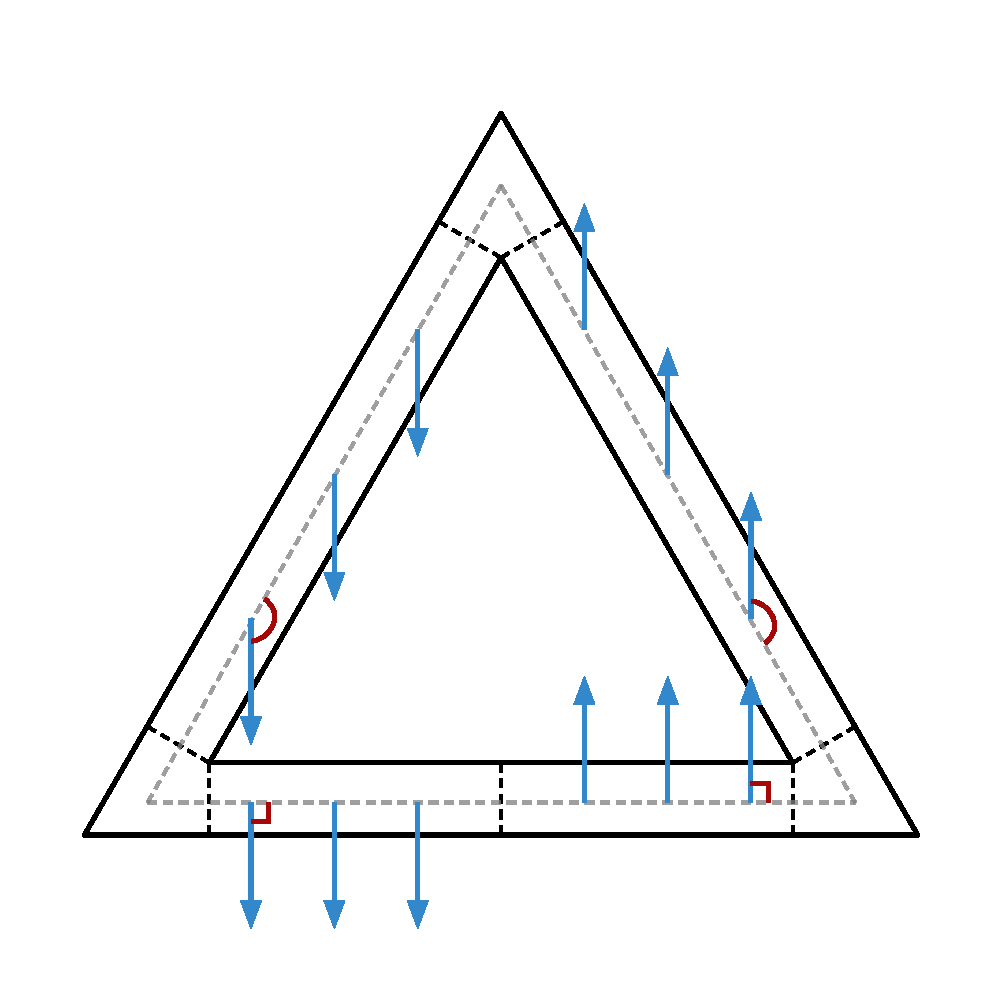
\includegraphics[width=0.5\textwidth]{./figures/triangular-island-vector-potential-divided.pdf}};
    \node[inner sep=0pt] (angle 1) at (-1.1,-1.1) {\small $\eta = -\dfrac{5\pi}{6}$};
    \node[inner sep=0pt] (angle 2) at (3.3,-1.0) {\small $\eta = \dfrac{5\pi}{6}$};
    \node[inner sep=0pt] (R1) at (-2.3,0.5) {\small I};
    \node[inner sep=0pt] (R2) at (2.3,0.5) {\small II};
    \node[inner sep=0pt] (R3) at (1.3,-3.3) {\small III};
    \node[inner sep=0pt] (R3) at (-1.3,-2.1) {\small IV};
  \end{tikzpicture}
  \caption{Triangular island with constant step function vector potential. The edges are divided up into four regions with differing vector potentials. Each segment is treated like a finite width ribbon where we can test its topology as function of $\mu$ and $\vec{A}$. Vector potential $\vec{A}$ makes an angle $\eta =  \mp \dfrac{5\pi}{6}, \pm \dfrac{\pi}{2}$, to each ribbon's main axis, respectively.}
  \label{fig: triangular-island-vector-potential-divided}
\end{figure}

The topological phase diagram for ribbons III and IV, with three rows, can be seen in Fig. \ref{subfig: majorana-number-y-axis}, we can see for varying $\mu$ and $A$, with $\vec{A} = A\hat{y}$, the system is topologically trivial (yellow) and nontrivial (blue).
It appears when the vector potential is perpendicular to the ribbon it does not contribute to the topology of the system.
Similarly, for ribbons I and II, with three rows, the topological phase diagram is seen in Fig. \ref{subfig: majorana-number-5pi6ths}.
Here the vector potential plays a vital role in transitioning the topology.

\begin{figure}[]
  \subfloat[\label{subfig: majorana-number-y-axis}]{%
    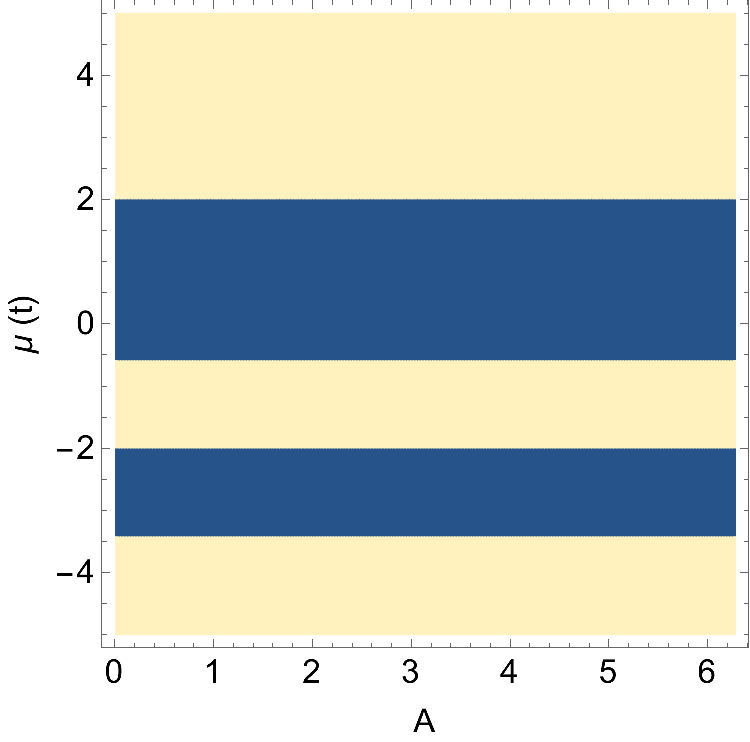
\includegraphics[width=0.3\textwidth]{./figures/majorana-number-y-axis.pdf}%
  }\hfill
  \subfloat[\label{subfig: majorana-number-5pi6ths}]{%
    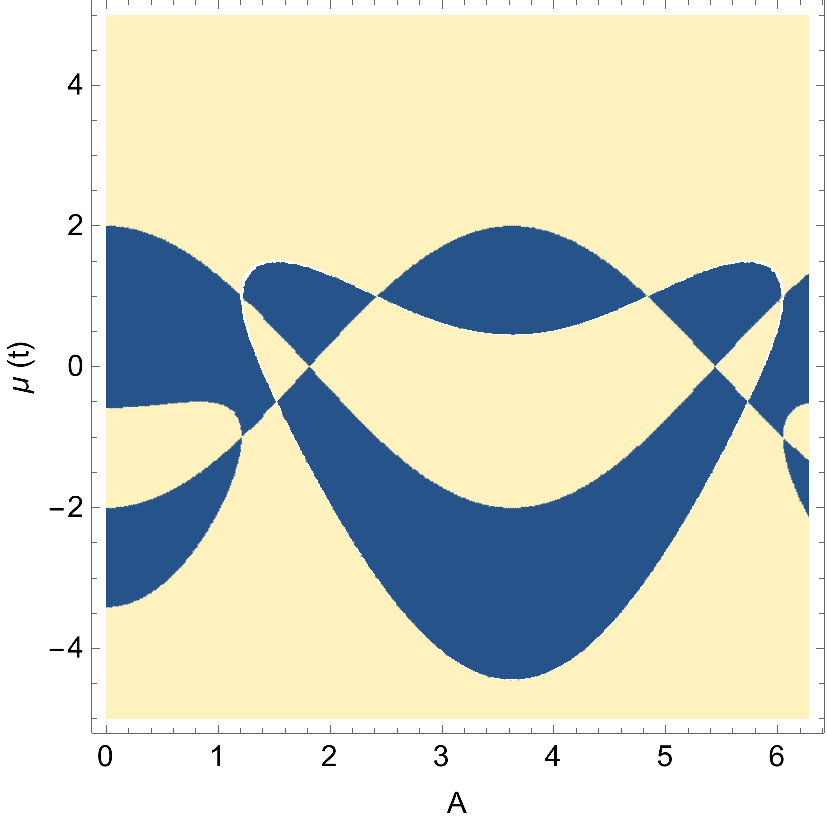
\includegraphics[width=0.3\textwidth]{./figures/majorana-number-5pi6ths.pdf}%
  }\hfill
  \caption{Topological phase diagrams for a system with three rows (a) regions III and IV, and (b) regions I and II, from Fig. \ref{fig: triangular-island-vector-potential-divided}}
  \label{fig: majorana-number}
\end{figure}

\begin{figure}[]
  \subfloat[\label{subfig: spectral-flow-mu-0.0}]{%
    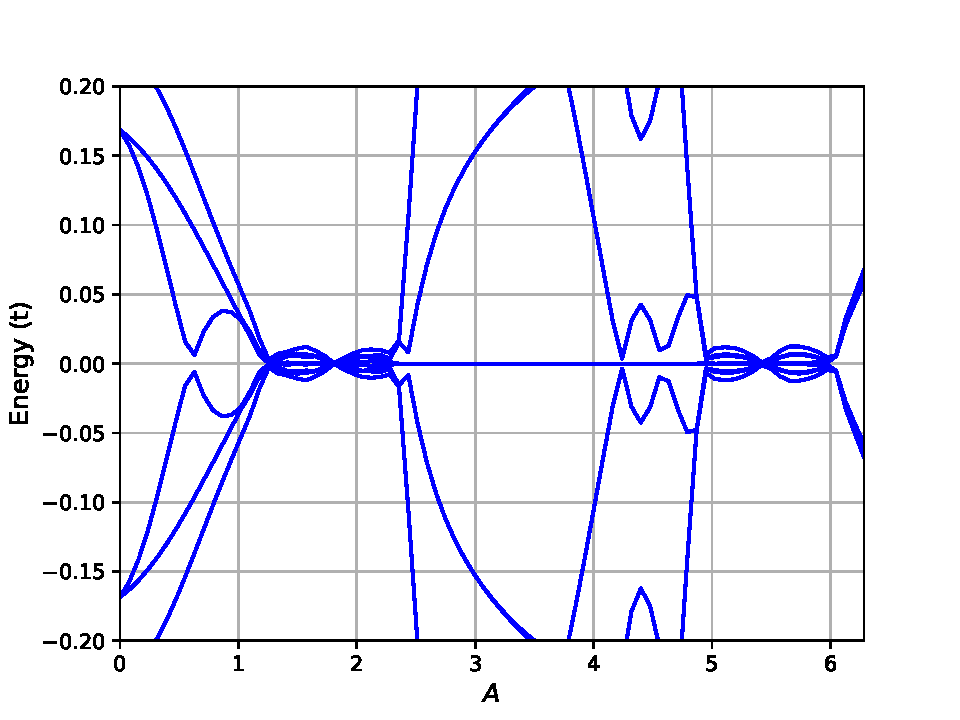
\includegraphics[width=0.3\textwidth]{./figures/spectral-flow-n-100-w-3-mu-0_0.pdf}%
  }\hfill
  \subfloat[\label{subfig: spectral-flow-mu-0.2}]{%
    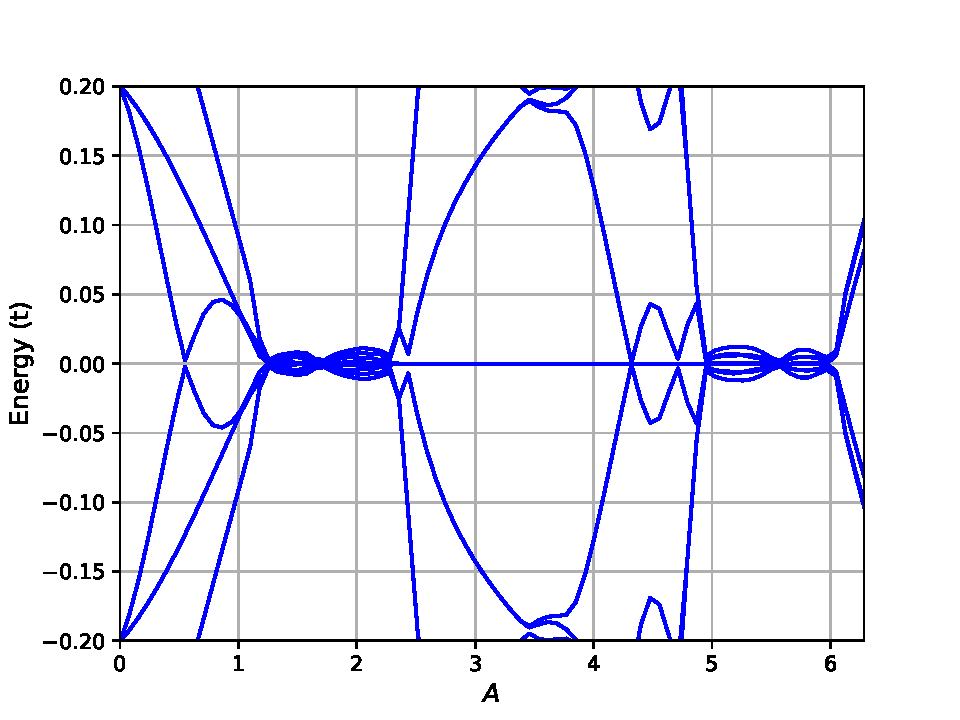
\includegraphics[width=0.3\textwidth]{./figures/spectral-flow-n-100-w-3-mu-0_2.pdf}%
  }\hfill
  \subfloat[\label{subfig: spectral-flow-mu-1.6}]{%
    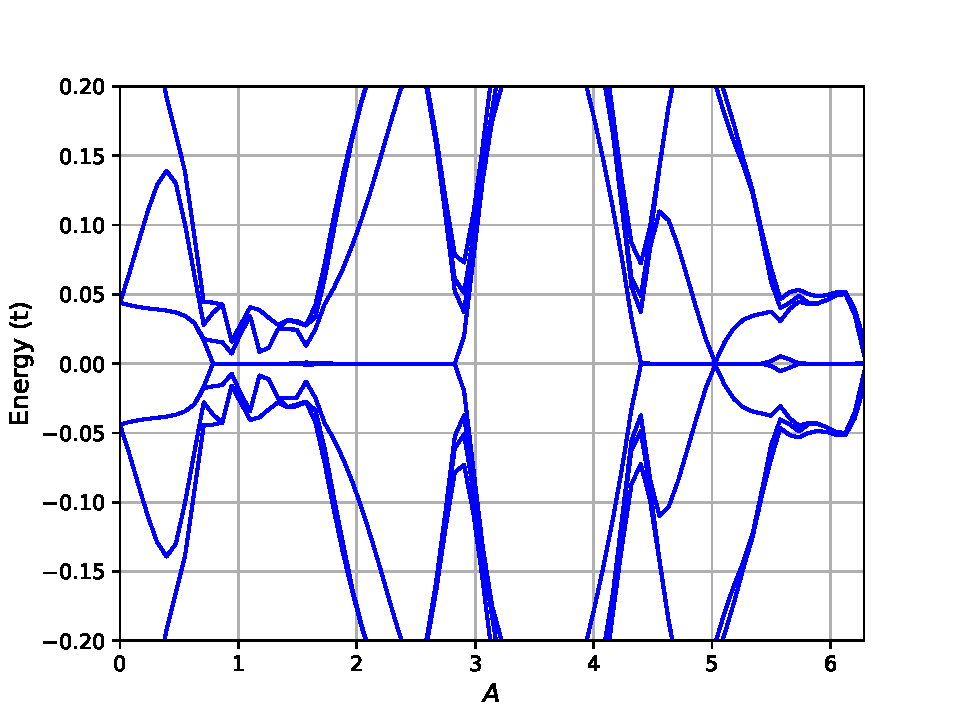
\includegraphics[width=0.3\textwidth]{./figures/spectral-flow-n-100-w-3-mu-1_6.pdf}%
  }\hfill
  \subfloat[\label{subfig: spectral-flow-mu-n1.6}]{%
    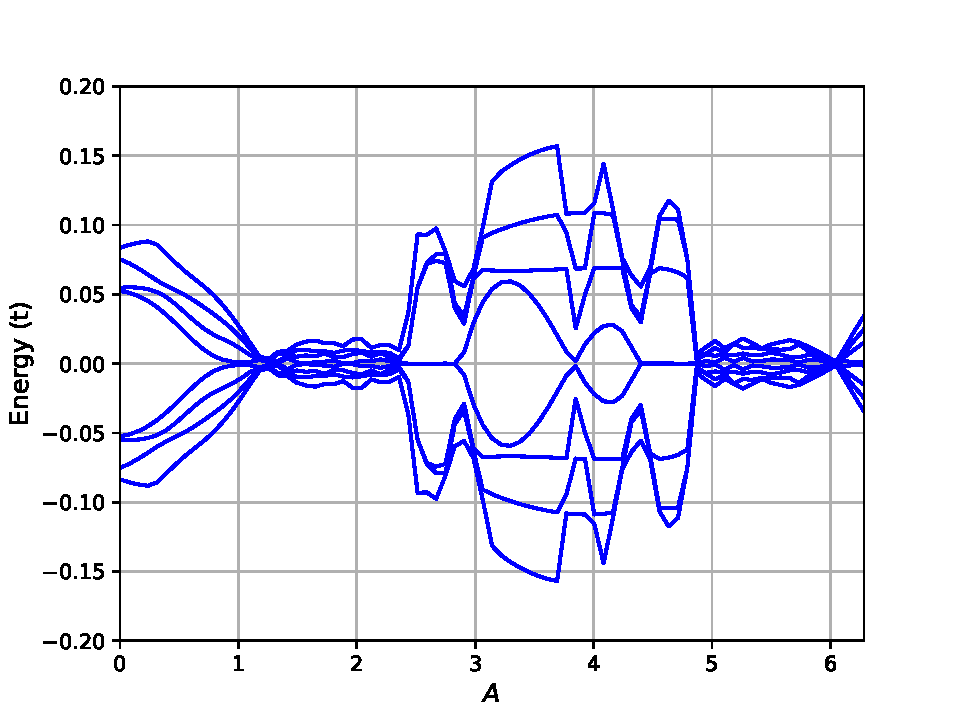
\includegraphics[width=0.3\textwidth]{./figures/spectral-flow-n-100-w-3-mu-n1_6.pdf}%
  }\hfill
  \caption{Eigenenergy spectral flow for a system with $n_r=100$ and $w_{edge}=3$, with (a) $\mu=0$, (b) $\mu=0.2t$, (c) $\mu=1.6t$, and (d) $\mu=-1.6t$.}
  \label{fig: spectral-flows}
\end{figure}

\begin{figure}[]
  \subfloat[\label{subfig: mzm-mu-0.0}]{%
    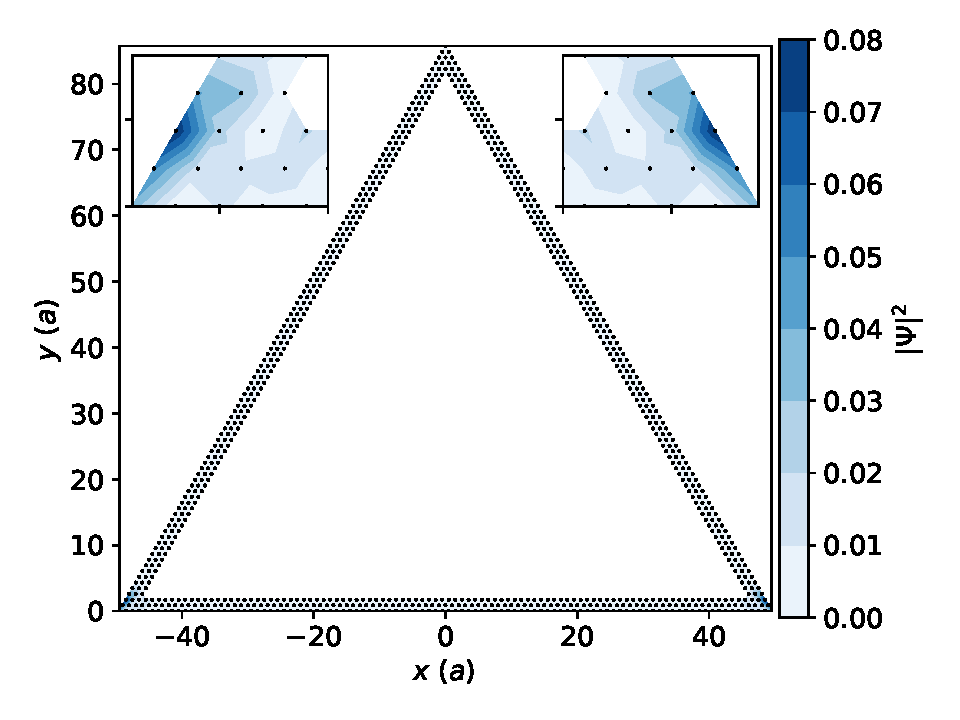
\includegraphics[width=0.3\textwidth]{./figures/En00-B-2_8274-n-100-w-3-mu-0_0.pdf}%
  }\hfill
  \subfloat[\label{subfig: mzm-mu-0.2}]{%
    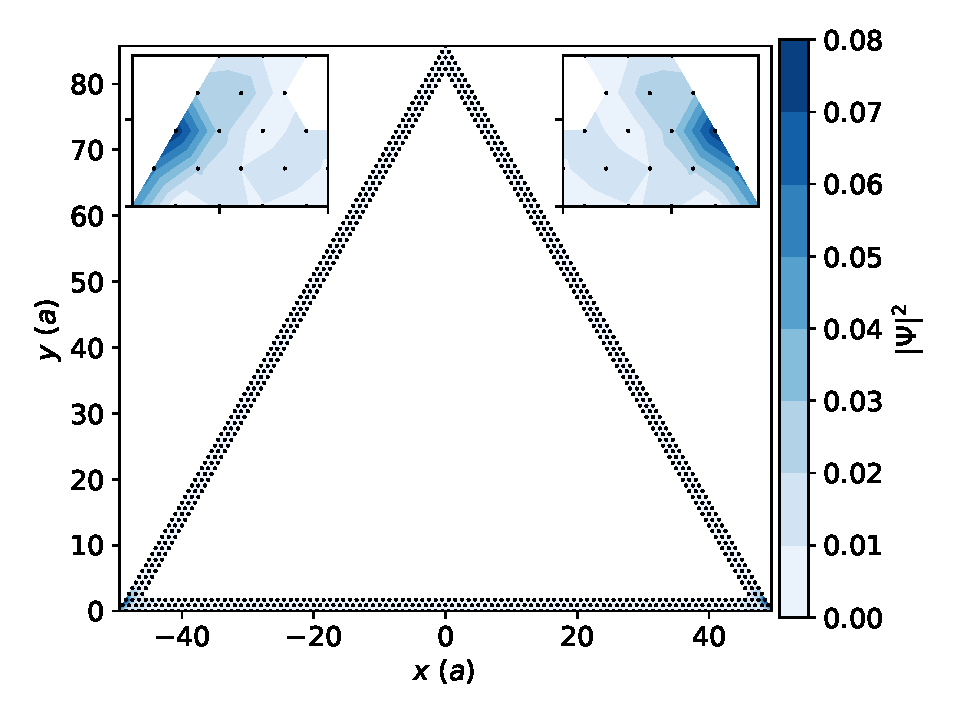
\includegraphics[width=0.3\textwidth]{./figures/En00-B-2_5918-n-100-w-3-mu-0_2.pdf}%
  }\hfill
  \subfloat[\label{subfig: mzm-mu-1.6}]{%
    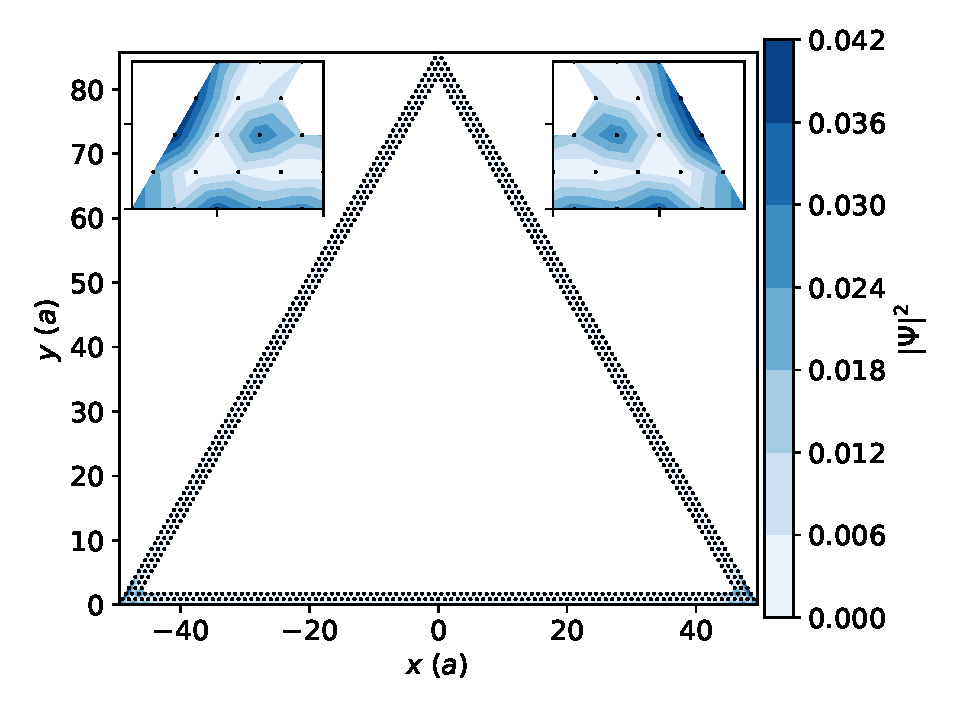
\includegraphics[width=0.3\textwidth]{./figures/En00-B-2_6704-n-100-w-3-mu-1_6.pdf}%
  }\hfill
  \subfloat[\label{subfig: mzm-mu-n1.6}]{%
    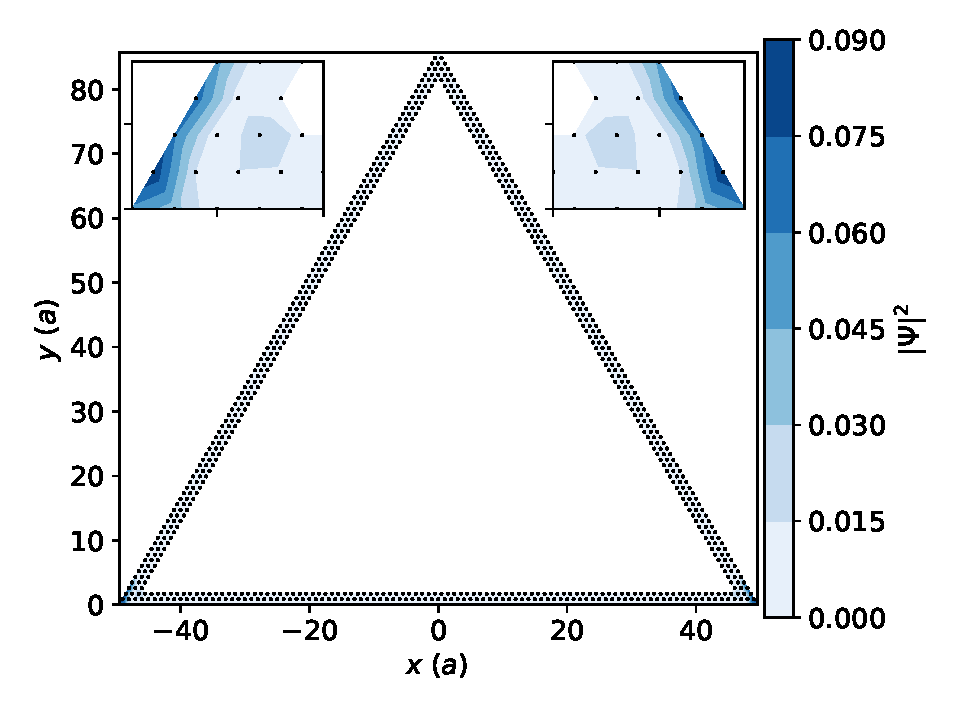
\includegraphics[width=0.3\textwidth]{./figures/En00-B-2_4347-n-100-w-3-mu-n1_6.pdf}%
  }\hfill
  \caption{MZMs for a system with $n_r=100$ and $w_{edge}=3$, with (a) $\mu=0.2t$, $A = 2.8274$, (b) $\mu=0.2t$, $A = 2.5918$, (c) $\mu=1.6t$, $A = 2.6704$, and (d) $\mu=-1.6t$, $A = 2.4347$.}
  \label{fig: mzm-wavefunctions}
\end{figure}

We make use of bulk-edge correspondence to justify MZMs hosting at the interfaces of the triangular islands edges, i.e. corners.
One simulataneously tunes regions I and II to be in a trivial(nontrivial) topological phase and regions III and IV to be nontrivial(trivial) topological phase, respectively.
To check we look at an eigenenergy spectral flow and eigenstates of a triangular lattice with size $n=100$, width $w=3$, and $A = [0,2\pi]$.
Fig. \ref{fig: spectral-flows} shows strong agreement of MZMs appearing in the same vector potential range as seen in Fig. \ref{subfig: majorana-number-5pi6ths}'s topological phase diagram.
As expected MZMs host at the bottom corners of the triangle where the differing topologies meet, as seen in Fig. \ref{fig: mzm-wavefunctions}.
We see a broad parameter space, $\mu$ and $A$, for our system to host MZMs.
Our calculations also show the MZMs live within a clean gap inside those parameter ranges.


\Red{For hollow triangles what are the advantages of using supercurrent/vector potential versus individually changing the chemical potential of each edges? For three-site triangles one can only control hopping since each site is shared by two edges.}

\section{Discussion and Conclusions}

How one can build this system warrants some thought.
A minimal model may be achieved by using a mesoscopic model involving quantum dots at the triangles vertices, to represent the minimal three point model \cite{dvirRealizationMinimalKitaev2023}.
If using epitaxial growth \cite{pietzschSpinResolvedElectronicStructure2006} one could make a network of vertex connected triangles, then either hollow the triangle out using ablation techniques or place a smaller inner voltage gates to tune the chemical potential to make a very strong trivial superconductor at its center.
One could place individual atoms using an STM tip \cite{schneiderPrecursorsMajoranaModes2022}.
Another option may be to use quasi-1D cuts on a QAHI with triangular lattice in proximity to an \textit{s}-wave superconductor \cite{xieCreatingLocalizedMajorana2021}.
To implement the inhomogeneous supercurrent or vector potential one could use a magnetic field and a uniform supercurrent or two antiparallel supercurrents separated by a 1D or quasi-1D insulator strip.
To braid MZMs in this system one only has to rotate and slowly turn on neighboring triangles inhomogeneous vector potentials to transition an edge to be of nontrivial topology.
The following schematic in Fig. \ref{fig: triangular-network-braiding} illustrates how such a manipulation of MZMs can occur.

\begin{figure}[]
  \begin{tikzpicture}
    \node[inner sep=0pt] (figure) at (0,0){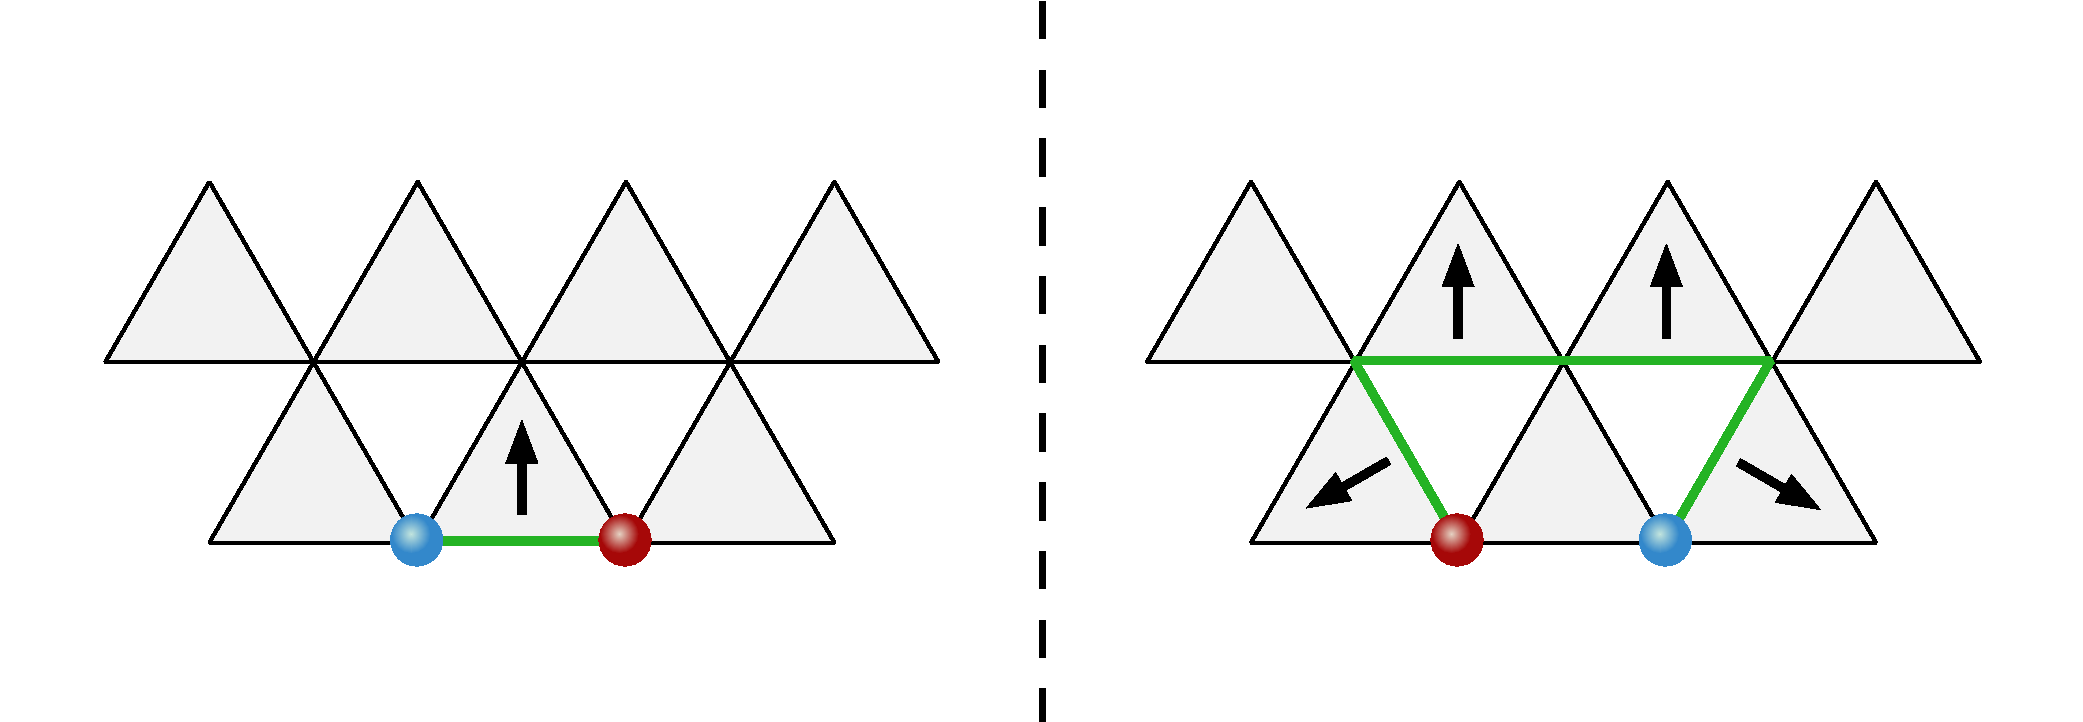
\includegraphics[width=0.5\textwidth]{./figures/triangle-network-braiding.pdf}};
    \node[inner sep=0pt] (gamma1) at (-2.7,-1.1) {\small $\gamma_1$};
    \node[inner sep=0pt] (gamma2) at (-1.8,-1.1) {\small $\gamma_2$};
    \node[inner sep=0pt] (gamma1') at (2.7,-1.1) {\small $\gamma_1$};
    \node[inner sep=0pt] (gamma2') at (1.8,-1.1) {\small $\gamma_2$};
  \end{tikzpicture}
  \caption{Network of tunable topological superconducting hollow triangular islands. The left panel shows the initialization of two MZMs $\gamma_1$ and $\gamma_2$. The right panel depicts the MZMs after a braiding operation. The arrows depict which island has an inhomogeneous vector potential applied and in general direction for a step-function. Green lines shows which edges are topologically nontrivial.}
  \label{fig: triangular-network-braiding}
\end{figure}

With the base model for a new platform displayed further work is still required.
A description of the Wannier states would be informative (\Blue{Hua, I'm not well versed in this type of description, could use your expertise here in writing this sentence as it sounds important to include}).
Perfectly fabricated devices are not always realistic, a further study of the effects misshapen lattice edges would be important to further gauge how robust our platform is.
Another calculation of how the MZMs evolve on a single triangle when the vector potential is rotated by $2\pi$ at its center would be informative if they survive such a process without mixing into higher order states and if they pick up a phase accumulation.

Would a uniform supercurrent or vector potential work?  Symmetry of the phase diagram under flipping sign of the vector potential. 

The three-site design may also make it convenient to implement parity readout by turning the third vertex temporily into a normal quantum dot and using the proposal in PRB 101, 235411. 

The bottom-up approach may also be favored due to the peripheral control circuit needed to precisely control the effective fermion Hamtiltonian also makes it convenient to distinguish MZMs from ABSs by implementing the various testing proposals.

\begin{acknowledgements}
  Supported by XYZ Grant No. XXXXXX etc.
\end{acknowledgements}


\bibliography{triag_cite}


\end{document}
